\documentclass[aspectratio=169]{beamer}
\usepackage[T1]{fontenc}
\usepackage{lmodern}
\usepackage{tikz}

% Brand colours: change these three to restyle the whole deck.
\definecolor{ink}{HTML}{14213D}
\definecolor{accent}{HTML}{FCA311}
\definecolor{paper}{HTML}{F5F5F2}

\setbeamercolor{background canvas}{bg=paper}
\setbeamercolor{normal text}{fg=ink}
\setbeamercolor{frametitle}{fg=ink}
\setbeamercolor{title}{fg=white}
\setbeamercolor{structure}{fg=accent}
\setbeamerfont{frametitle}{size=\LARGE, series=\bfseries}
\setbeamertemplate{navigation symbols}{}
\setbeamertemplate{itemize item}{\textcolor{accent}{\rule[0.3ex]{0.6em}{0.6em}}}
\setbeamertemplate{frametitle}{\vspace{1.2em}\insertframetitle\par\vspace{-0.2em}\textcolor{accent}{\rule{2cm}{3pt}}}
\setbeamertemplate{footline}{\hfill\textcolor{ink!50}{\footnotesize GreenLoop \quad \insertframenumber}\hspace{1.5em}\vspace{1em}}

% A big number with a label, for the traction slide.
\newcommand{\bigstat}[2]{\begin{minipage}{0.3\textwidth}\centering{\fontsize{34}{38}\selectfont\bfseries\textcolor{accent}{#1}}\\[0.3em]#2\end{minipage}}

\begin{document}

{
\setbeamercolor{background canvas}{bg=ink}
\begin{frame}[plain]
  \vfill
  {\fontsize{40}{44}\selectfont\bfseries\textcolor{white}{GreenLoop}}\\[0.6em]
  {\Large\textcolor{accent}{Reusable packaging for local food delivery}}\\[2em]
  \textcolor{white}{Project proposal, seed round, September 2026}
  \vfill
\end{frame}
}

\begin{frame}{The problem}
  \begin{itemize}
    \item A typical delivery order creates 6 pieces of single use packaging.
    \item Restaurants pay for it twice: to buy it and to meet waste rules.
    \item Customers say they want an alternative, but none is convenient.
  \end{itemize}
\end{frame}

\begin{frame}{Our solution}
  \begin{columns}[c]
    \begin{column}{0.5\textwidth}
      Sturdy containers with a deposit. Couriers collect empties on their next drop in the same street, and we wash them in a shared hub.
    \end{column}
    \begin{column}{0.45\textwidth}
      \centering
      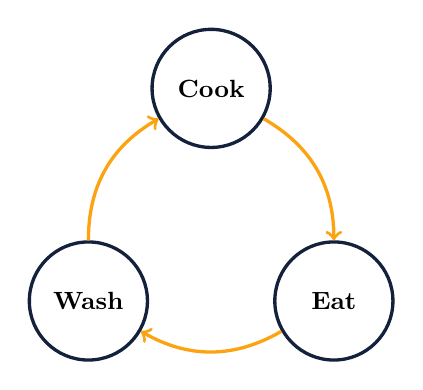
\begin{tikzpicture}[every node/.style={circle, draw=ink, very thick, fill=white, minimum size=1.5cm, font=\small\bfseries}]
        \node (r) at (90:1.8) {Cook};
        \node (c) at (330:1.8) {Eat};
        \node (h) at (210:1.8) {Wash};
        \draw[->, very thick, accent] (r) to[bend left] (c);
        \draw[->, very thick, accent] (c) to[bend left] (h);
        \draw[->, very thick, accent] (h) to[bend left] (r);
      \end{tikzpicture}
    \end{column}
  \end{columns}
\end{frame}

\begin{frame}{Traction so far}
  \vspace{1em}
  \centering
  \bigstat{22}{partner restaurants}\hfill
  \bigstat{9{,}400}{containers reused}\hfill
  \bigstat{93\%}{return rate}
\end{frame}

\begin{frame}{Roadmap}
  \centering
  % Edit the quarters and milestones.
  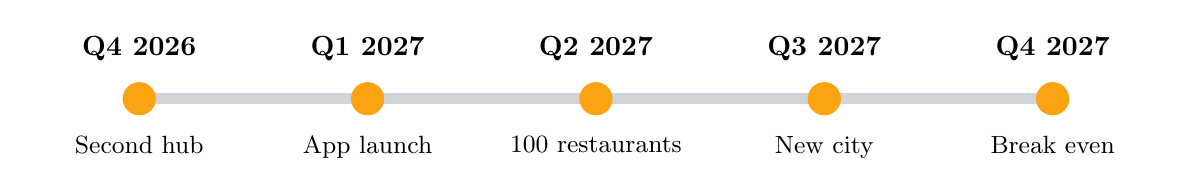
\begin{tikzpicture}[x=2.9cm]
    \draw[line width=4pt, ink!20] (0,0) -- (4,0);
    \foreach \i/\q/\m in {0/Q4 2026/Second hub, 1/Q1 2027/App launch, 2/Q2 2027/100 restaurants, 3/Q3 2027/New city, 4/Q4 2027/Break even} {
      \fill[accent] (\i,0) circle (6pt);
      \node[above=10pt, font=\bfseries] at (\i,0) {\q};
      \node[below=10pt, text width=2.6cm, align=center, font=\small] at (\i,0) {\m};
    }
  \end{tikzpicture}
\end{frame}

\begin{frame}{Budget and ask}
  \begin{columns}[T]
    \begin{column}{0.5\textwidth}
      \begin{tabular}{lr}
        Containers & 120k \\
        Washing hub & 90k \\
        Software & 60k \\
        Team, 12 months & 230k \\
        \hline
        \textbf{Total} & \textbf{500k} \\
      \end{tabular}
    \end{column}
    \begin{column}{0.45\textwidth}
      
\begin{tikzpicture}
        \node[fill=ink, text=white, rounded corners=6pt, inner sep=1em, text width=0.8\textwidth, align=center]
          {{\Large\bfseries We are raising 500k}\\[0.4em] to reach two cities by 2027.};
      \end{tikzpicture}
    \end{column}
  \end{columns}
\end{frame}

{
\setbeamercolor{background canvas}{bg=accent}
\begin{frame}[plain]
  \centering\vfill
  {\fontsize{36}{40}\selectfont\bfseries\textcolor{ink}{Let's close the loop.}}\\[1em]
  \textcolor{ink}{hello@greenloop.example \quad +00 000 000 000}
  \vfill
\end{frame}
}

\end{document}
